%%%%%%%%%%%%%%%%%%%%%%%%%%%%%%%%%%%%%%%%%%%
%
% From a template maintained at https://github.com/jamesrobertlloyd/cbl-tikz-poster
%
% Code near the top should be fairly standard and not need to be changed
%  - except for the document class
% Code lower down is more likely to be customised
%
%%%%%%%%%%%%%%%%%%%%%%%%%%%%%%%%%%%%%%%%%%%

%%%%%%%%%%%%%%%%%%%%%%%%%%%%%%%%%%%%%%%%%%%
%
% Document class
%
% Change this if you want a different size / orientation poster etc
%
%%%%%%%%%%%%%%%%%%%%%%%%%%%%%%%%%%%%%%%%%%%

\documentclass[landscape,a0b,final,a4resizeable]{a0poster}
%\documentclass[portrait,a0b,final,a4resizeable]{a0poster}

%%%%%%%%%%%%%%%%%%%%%%%%%%%%%%%%%%%%%%%%%%%
%
% 'Basic' packages
%
% TODO - Almost certainly some are unnecessary - feel free to remove nonstandard
% packages if you think it is a good idea not to always have them
%
%%%%%%%%%%%%%%%%%%%%%%%%%%%%%%%%%%%%%%%%%%%

\usepackage{multicol}
\usepackage{color}
\usepackage{shadow}
\usepackage{morefloats}
\usepackage{cite}
\usepackage[pdftex]{graphicx}
\usepackage{rotating}
\usepackage{amsmath, amsthm, amssymb, bm}
\usepackage{array}
\usepackage{nth}
\usepackage[square,numbers]{natbib}
\usepackage{booktabs}

%%%%%%%%%%%%%%%%%%%%%%%%%%%%%%%%%%%%%%%%%%%
%
% TIKZ packages and common definitions
%
% Add extra things as per your tikz needs
%
%%%%%%%%%%%%%%%%%%%%%%%%%%%%%%%%%%%%%%%%%%%

\usepackage{../common/picins}
\usepackage{tikz}
\usetikzlibrary{shapes.geometric,arrows,chains,matrix,positioning,scopes,calc}
\tikzstyle{mybox} = [draw=white, rectangle]

%%%%%%%%%%%%%%%%%%%%%%%%%%%%%%%%%%%%%%%%%%%
%
% myfig
%
% \myfig - replacement for \figure
% necessary, since in multicol-environment 
% \figure won't work        
%                 
%%%%%%%%%%%%%%%%%%%%%%%%%%%%%%%%%%%%%%%%%%%

\newcommand{\myfig}[3][0]{
\begin{center}
  \vspace{1.5cm}
  \includegraphics[width=#3\hsize,angle=#1]{#2}
  \nobreak\medskip
\end{center}}

%%%%%%%%%%%%%%%%%%%%%%%%%%%%%%%%%%%%%%%%%%%
%
% mycaption                
%
% \mycaption - replacement for \caption
% necessary, since in multicol-environment \figure and
% therefore \caption won't work
%
%%%%%%%%%%%%%%%%%%%%%%%%%%%%%%%%%%%%%%%%%%%

%\newcounter{figure}
\setcounter{figure}{1}
\newcommand{\mycaption}[1]{
  \vspace{0.5cm}
  \begin{quote}
    {{\sc Figure} \arabic{figure}: #1}
  \end{quote}
  \vspace{1cm}
  \stepcounter{figure}
}

%%%%%%%%%%%%%%%%%%%%%%%%%%%%%%%%%%%%%%%%%%%
%
% Some standard colours
%
%%%%%%%%%%%%%%%%%%%%%%%%%%%%%%%%%%%%%%%%%%%

\definecolor{camlightblue}{rgb}{0.601 , 0.8, 1}
\definecolor{camdarkblue}{rgb}{0, 0.203, 0.402}
\definecolor{camred}{rgb}{1, 0.203, 0}
\definecolor{camyellow}{rgb}{1, 0.8, 0}
\definecolor{lightblue}{rgb}{0, 0, 0.80}
\definecolor{white}{rgb}{1, 1, 1}
\definecolor{whiteblue}{rgb}{0.80, 0.80, 1}

%%%%%%%%%%%%%%%%%%%%%%%%%%%%%%%%%%%%%%%%%%%
%
% Some look and feel definitions
%
%%%%%%%%%%%%%%%%%%%%%%%%%%%%%%%%%%%%%%%%%%%

\setlength{\columnsep}{0.03\textwidth}
\setlength{\columnseprule}{0.0018\textwidth}
\setlength{\parindent}{0.0cm}

%%%%%%%%%%%%%%%%%%%%%%%%%%%%%%%%%%%%%%%%%%%
%
% \mysection - replacement for \section*
% 
% Puts a pretty box around some text
% TODO - any other thoughts for what this box should look like
%
%%%%%%%%%%%%%%%%%%%%%%%%%%%%%%%%%%%%%%%%%%%

\tikzstyle{mysection} = [rectangle, 
									draw=none, 
									shade, 
									outer color=camlightblue!30,
									inner color=camlightblue!30,
									text width=0.965\columnwidth,
									text centered,
									rounded corners=20pt,
									minimum height=0.11\columnwidth]

\newcommand{\mysection}[1]
{
\begin{center}
  \begin{tikzpicture}
    \node[mysection] {\sffamily\bfseries\LARGE#1};
  \end{tikzpicture}
\end{center}
}

%%%%%%%%%%%%%%%%%%%%%%%%%%%%%%%%%%%%%%%%%%%
%
% Set the font
%
% TODO - Not sure what a canonical choice is - feel free to modify
%
%%%%%%%%%%%%%%%%%%%%%%%%%%%%%%%%%%%%%%%%%%%

\renewcommand{\familydefault}{cmss}
\sffamily

%%%%%%%%%%%%%%%%%%%%%%%%%%%%%%%%%%%%%%%%%%%
%
% Poster environment
%
% Centres everything and can be used to define the width of the content
%
%%%%%%%%%%%%%%%%%%%%%%%%%%%%%%%%%%%%%%%%%%%

\newenvironment{poster}{
  \begin{center}
  \begin{minipage}[c]{0.96\textwidth}
}{
  \end{minipage} 
  \end{center}
}

%%%%%%%%%%%%%%%%%%%%%%%%%%%%%%%%%%%%%%%%%%%
%
% This is probably a good place to put content specific packages and definitions
%
%%%%%%%%%%%%%%%%%%%%%%%%%%%%%%%%%%%%%%%%%%%

\newtheorem{thm}{Theorem}%[section]
\newtheorem{lem}[thm]{Lemma}
\newtheorem{prop}[thm]{Proposition}
\newtheorem{cor}[thm]{Corollary}

\newtheorem*{theorem*}{Theorem}

\theoremstyle{definition}
\newtheorem*{definition*}{Definition}
\newtheorem{definition}[thm]{Definition}%[section]
\newtheorem{conj}{Conjecture}[section]
\newtheorem{exmp}{Example}[section]
\newtheorem{rem}[thm]{Remark}

\theoremstyle{remark}
%\newtheorem{rem}{Remark}
\newtheorem{note}{Note}
\newtheorem{case}{Case}

\newcommand{\eqd}{\overset{\,_{\!d}}{=}}
\newcommand{\defn}[1]{\emph{#1}}

\newcommand{\Law}{\mathcal{L}}

\def\given{\,|\,}

\def\SGinf{\mathbb{S}_{\infty}}

\newcommand{\NonNegInts}{\mathbb{Z}_+}
\newcommand{\Nats}{\mathbb{N}}
\newcommand{\Rationals}{\mathbb{Q}}
\newcommand{\Reals}{\mathbb{R}}

\newcommand{\as}{\textrm{a.s.}}

\def\[#1\]{\begin{align}#1\end{align}}
\newcommand{\defas}{:=}

\newcommand{\Normal}{\mathcal{N}}
\newcommand{\dist}{\ \sim\ }

\newcommand{\kernel}{\kappa}
\newcommand{\kernelmatrix}{K}
\newcommand{\scalefactor}{s}
\newcommand{\lengthscale}{\ell}
\newcommand{\targets}{T}
\newcommand{\noise}{\sigma_\targets}
\newcommand{\pseudopoints}{\eta}
\newcommand{\inputpoints}{\xi}
\newcommand{\covhyppar}{\psi}
\newcommand{\logistic}{\phi}

\newcommand{\CompOrder}{\mathcal{O}}
\def\graphspace{\mathbf{G}}
\def\Uniform{\mbox{\rm Uniform}}
\def\Bernoulli{\mbox{\rm Bernoulli}}
\def\ie{i.e.,\ }
\def\eg{e.g.,\ }
\def\iid{i.i.d.\ }
\def\simiid{\sim_{\mbox{\tiny iid}}}
\def\simind{\sim_{\mbox{\tiny ind}}}
\def\eqdist{\stackrel{\mbox{\tiny d}}{=}}
\def\ahfunction{\theta}       
\def\AHfunction{\Theta}           % A-H random function
\def\AHvar{U}                     % A-H uniform variables
\def\AHvaralt{V}                  % A-H uniform variables - for bipartite data
\def\larray{W}                    % latent array sampled with A-H
%\def\latentspace{\mathbf{W}}      % range of entries
\def\latentspace{\mathcal{W}}      % range of entries
\def\darray{X}                    % data array
%\def\dataspace{\mathbf{X}}        % sample space
\def\dataspace{\mathcal{X}}        % sample space
\def\cfspace{\mathbf{C}}          % space of continuous functions
%\def\GP{\mbox{\mathcal{GP}}}
\def\GP{\mathcal{GP}}
\def\likelihood{P}
\def\CovData{C}
\def\CovDataAlt{D}

\def\newarrow{\mbox{\begin{tikzpicture}
             \useasboundingbox{(-3pt,-4.5pt) rectangle (19pt,1pt)};
             \draw[->] (0,-0.07)--(17pt,-0.07);\end{tikzpicture}}}

%%%%%%%%%%%%%%%%%%%%%%%%%%%%%%%%%%%%%%%%%%%
%
% The document environment starts here
%
%%%%%%%%%%%%%%%%%%%%%%%%%%%%%%%%%%%%%%%%%%%

\begin{document}

%%%%%%%%%%%%%%%%%%%%%%%%%%%%%%%%%%%%%%%%%%%
%
% Begin the poster environment - centres things and potentially changes the width
%
%%%%%%%%%%%%%%%%%%%%%%%%%%%%%%%%%%%%%%%%%%%

\begin{poster}

%%%%%%%%%%%%%%%%%%%%%%%%%%%%%%%%%%%%%%%%%%%
%
% Potentially add some space at the top of the poster
%
%%%%%%%%%%%%%%%%%%%%%%%%%%%%%%%%%%%%%%%%%%%

\vspace{0\baselineskip}

%%%%%%%%%%%%%%%%%%%%%%%%%%%%%%%%%%%%%%%%%%%
%
% Draw the header as a TIKZ picture
%
% Using TIKZ to allow for easy alignment
%
%%%%%%%%%%%%%%%%%%%%%%%%%%%%%%%%%%%%%%%%%%%

\begin{center}
\begin{tikzpicture}[x=0.5\textwidth]
    % Dummy nodes at edges for spacing
    % TODO - a better way?
    \node at (+1, 0) {};    
    \node at (-1, 0) {};
    % Set the size of the badges
    \def \badgeheight {0.08\textwidth}
    % Title text
    \node[inner sep=0,text width=0.5\textwidth,text centered,font=\Huge] (Title) at (0,0) 
    {
      {\sffamily \Huge \textbf{Estimating Convergence of Markov chains with\\\(L\)-Lag Couplings}}\\
      {\huge\sffamily Niloy Biswas\textsuperscript{1}, Pierre E. Jacob\textsuperscript{1}, Paul Vanetti\textsuperscript{2}}\\
      \vspace{-0.3\baselineskip}
      {\large\sffamily 1: Department of Statistics, Harvard University 2: Department of Statistics, University of Oxford}
    };
    % Harvard badge
    \node [mybox] (Cambridge Badge) at (-0.9, 0) {
        
\includegraphics[height=0.125\textwidth]{../badges/harvard.png}
    };
    % Oxford badge
    \node [mybox] (box) at (0.875, 0) {
        
\includegraphics[width=0.125\textwidth]{../badges/oxford.png}
    };
\end{tikzpicture}
\end{center}

%%%%%%%%%%%%%%%%%%%%%%%%%%%%%%%%%%%%%%%%%%%
%
% Spacing between title and main body
%
%%%%%%%%%%%%%%%%%%%%%%%%%%%%%%%%%%%%%%%%%%%

\vspace{1\baselineskip}

%%%%%%%%%%%%%%%%%%%%%%%%%%%%%%%%%%%%%%%%%%%
%
% Columns environment
%
%%%%%%%%%%%%%%%%%%%%%%%%%%%%%%%%%%%%%%%%%%%

\begin{multicols}{3}

%%%%%%%%%%%%%%%%%%%%%%%%%%%%%%%%%%%%%%%%%%%
%
% Start of content
%
%%%%%%%%%%%%%%%%%%%%%%%%%%%%%%%%%%%%%%%%%%%

\large

\mysection{Motivation: finite-time bias of MCMC}

\vspace{1\baselineskip}

{\Large \begin{itemize}
\item MCMC methods have \textbf{non-asymptotic bias}: they only reach the target distribution as the number of iterations goes to infinity.
\vspace{1\baselineskip}
\item We introduce \textbf{\(L\)-lag couplings} to generate computable, non-asymptotic upper bound estimates for the total variation or the Wasserstein distance of general Markov chains.
\end{itemize}}

%\begin{center}
%\begin{tikzpicture}
  \begin{scope}[yshift=0\textwidth]
    \begin{scope}[xshift=0cm]
      \node [mybox] (box){
        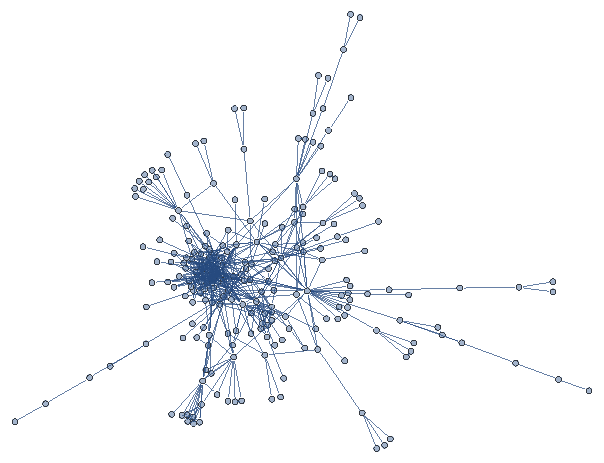
\includegraphics[width=0.15\textwidth]{../misc/graph_standard.pdf}
      };
    \end{scope}
    \begin{scope}[xshift=0.14\textwidth]
      \node [mybox] (box){
        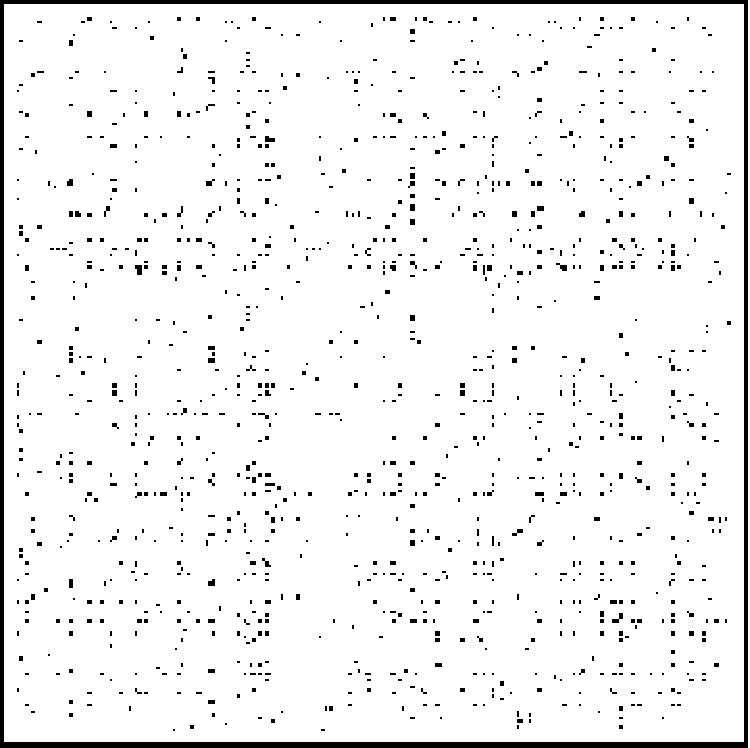
\includegraphics[width=0.12\textwidth]{../misc/unsorted_adjacency_matrix.pdf}
      };
    \end{scope}
  \end{scope}
  \begin{scope}[yshift=-0.08\textwidth]
    \begin{scope}[xshift=0cm]
        \node[inner sep=0,text width=0.13\textwidth, text centered] (note1) at (0,0) {
         \Large A protein interactome\ldots};
     \end{scope}
    \begin{scope}[xshift=0.14\textwidth]
        \node[inner sep=0,text width=0.13\textwidth, text centered] (note1) at (0,0) {
         \Large \ldots encoded as an array};
     \end{scope}
  \end{scope}
\end{tikzpicture}

%\end{center}

\vspace{1\baselineskip}

{\Large 
\begin{itemize}
\item We apply \(L\)-lag couplings to:
\vspace{0.5\baselineskip}
\begin{itemize}
\item Determine MCMC burn-in
\vspace{0.5\baselineskip}
\item Compare different MCMC algorithms with the same target
\vspace{0.5\baselineskip}
\item Compare exact and approximate MCMC
\end{itemize}
\end{itemize}}

%\begin{center}
%\begin{tikzpicture}
  \begin{scope}[yshift=0\textwidth]
    \begin{scope}[xshift=0cm]
      \node [mybox] (box){
        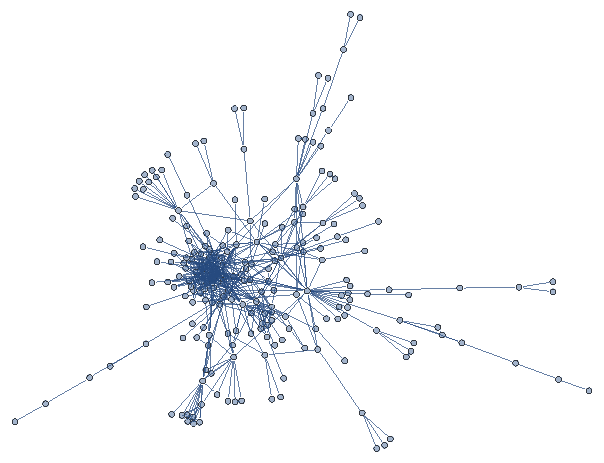
\includegraphics[width=0.15\textwidth]{../misc/graph_standard.pdf}
      };
    \end{scope}
    \begin{scope}[xshift=0.14\textwidth]
      \node [mybox] (box){
        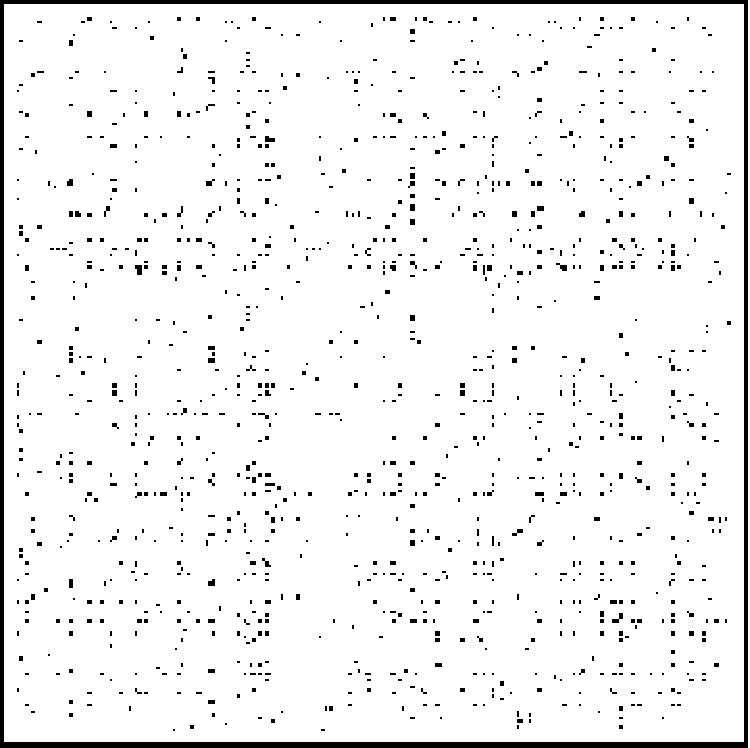
\includegraphics[width=0.12\textwidth]{../misc/unsorted_adjacency_matrix.pdf}
      };
    \end{scope}
  \end{scope}
  \begin{scope}[yshift=-0.08\textwidth]
    \begin{scope}[xshift=0cm]
        \node[inner sep=0,text width=0.13\textwidth, text centered] (note1) at (0,0) {
         \Large A protein interactome\ldots};
     \end{scope}
    \begin{scope}[xshift=0.14\textwidth]
        \node[inner sep=0,text width=0.13\textwidth, text centered] (note1) at (0,0) {
         \Large \ldots encoded as an array};
     \end{scope}
  \end{scope}
\end{tikzpicture}

%\end{center}

\vspace{2\baselineskip}


\mysection{What are \(L\)-Lag Couplings?}

\vspace{1\baselineskip}

{\Large \begin{itemize}
\item A pair of Markov chains \((X_t, Y_t)_{t \geq 0}\) such that:
\vspace{0.5\baselineskip}
\begin{itemize}
\item Same marginal distributions: 
\( X_t \sim Y_t \sim \pi_t \ \forall t \geq 0 \ \text{ with } \pi_t \overset{t \rightarrow \infty}{\Rightarrow} \pi \)
\item \(X_t\) and \(Y_{t-L}\) meet \textit{\underline{exactly}} at time 
\(\tau^{(L)}:= inf \{ t > L : X_t = Y_{t-L} \} \)
\end{itemize}
\end{itemize}}

\vspace{1\baselineskip}

\begin{center}
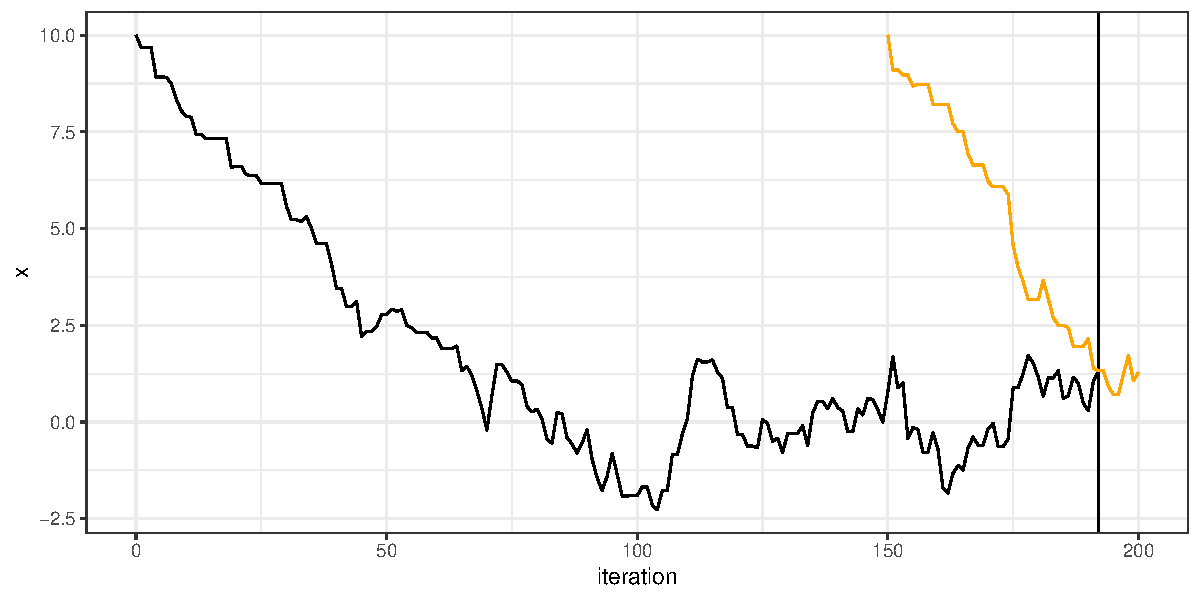
\includegraphics[width=0.275\paperwidth]{../misc/rwmh_standard_normal_lag_150_trajectory.pdf}
\end{center}


%\begin{center}
%\begin{tikzpicture}
  \begin{scope}[yshift=0cm]
    \tikzstyle{graph_node}=[circle,minimum size=0.014\textwidth,inner sep=0pt, fill=camlightblue]
    \def \radius {0.045\textwidth}
    \begin{scope}[xshift=0cm]
      \foreach \s in {1,...,10}
      {
        \node[draw, graph_node] (N\s) at ({360/10 * (\s - 1) + 90}:\radius) {\s};
      }   
      \path (N2) edge (N6);
      \path (N4) edge (N9);
      \path (N5) edge (N6);
      \path (N5) edge (N8);
      \path (N7) edge (N8);
      \path (N8) edge (N9);
      \path (N8) edge (N10);
      \path (N9) edge (N10);
    \end{scope}
    \begin{scope}[xshift=0.14\textwidth]
      \def \s {1}
      \node[draw, graph_node] (N\s) at ({360/10 * (\s - 1) + 90}:\radius) {2};
      \def \s {2}
      \node[draw, graph_node] (N\s) at ({360/10 * (\s - 1) + 90}:\radius) {7};
      \def \s {3}
      \node[draw, graph_node] (N\s) at ({360/10 * (\s - 1) + 90}:\radius) {6};
      \def \s {4}
      \node[draw, graph_node] (N\s) at ({360/10 * (\s - 1) + 90}:\radius) {5};
      \def \s {5}
      \node[draw, graph_node] (N\s) at ({360/10 * (\s - 1) + 90}:\radius) {3};
      \def \s {6}
      \node[draw, graph_node] (N\s) at ({360/10 * (\s - 1) + 90}:\radius) {1};
      \def \s {7}
      \node[draw, graph_node] (N\s) at ({360/10 * (\s - 1) + 90}:\radius) {10};
      \def \s {8}
      \node[draw, graph_node] (N\s) at ({360/10 * (\s - 1) + 90}:\radius) {8};
      \def \s {9}
      \node[draw, graph_node] (N\s) at ({360/10 * (\s - 1) + 90}:\radius) {4};
      \def \s {10}
      \node[draw, graph_node] (N\s) at ({360/10 * (\s - 1) + 90}:\radius) {9};
      \path (N2) edge (N6);
      \path (N4) edge (N9);
      \path (N5) edge (N6);
      \path (N5) edge (N8);
      \path (N7) edge (N8);
      \path (N8) edge (N9);
      \path (N8) edge (N10);
      \path (N9) edge (N10);
    \end{scope}
    \begin{scope}[xshift=0.07\textwidth]
      \node[inner sep=0,text width=0.13\textwidth, text centered,font=\Huge] (note1) at (0,0) {
         $\equiv$};
    \end{scope}
  \end{scope}
  \begin{scope}[yshift=-0.14\textwidth]
    \begin{scope}[xshift=0cm]
      \node [mybox] (box){
        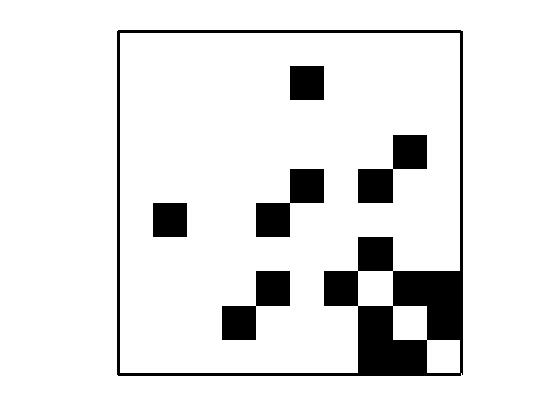
\includegraphics[width=0.15\textwidth]{../misc/adj.png}
      };
    \end{scope}
    \begin{scope}[xshift=0.14\textwidth]
      \node [mybox] (box){
        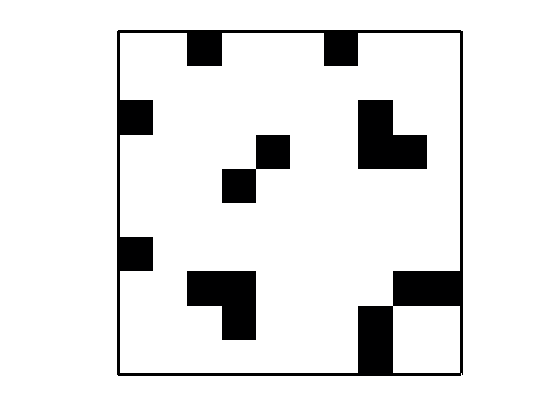
\includegraphics[width=0.15\textwidth]{../misc/adj_perm.png}
      };
    \end{scope}
    \begin{scope}[xshift=0.07\textwidth]
      \node[inner sep=0,text width=0.13\textwidth, text centered,font=\Huge] (note1) at (0,0) {
         $\equiv$};
    \end{scope}
  \end{scope}
\end{tikzpicture}

%\end{center}

\vspace{\baselineskip}

%\begin{center}
%{\Large When the labelling of nodes is arbitrary, the two adjacency matrices should be treated equivalently.}
%\end{center}

\vspace{2\baselineskip}

\newpage

\mysection{Main Theorem}

\vspace{1\baselineskip}

\begin{Theorem}
Consider an \(L\)-lag coupling of chains \((X_t, Y_t)_{t \geq 0}\), where \( X_t \overset{t \rightarrow \infty}{\Rightarrow} \pi\) and 
meeting time \(\tau^{(L)}:= inf \{ t > L : X_t = Y_{t-L} \} \) has sub-exponential tails. Then, 
\begin{equation}
d_{\text{TV}}(\pi_t, \pi) \leq  \mathbb{E} \Big[ \max(0, \bigl\lceil \frac{\tau^{(L)} - L -t}{L} \bigr\rceil) \Big]
\end{equation}
Further assume for some \(\eta >0\), \((2+\eta)\)-moments of chain \((X_t)_{t \geq 0}\) are uniformly bounded. Then, 
\begin{equation}
d_{\text{W}}(\pi_t, \pi) \leq   \mathbb{E} \Big[ \sum_{j=1}^{ \bigl\lceil \frac{\tau^{(L)} - L -t}{L} \bigr\rceil }  \| X_{t+jL} - Y_{t+(j-1)L} \|_1 \Big]
\end{equation}
\end{Theorem}


%\begin{definition*}
%  An array $\darray=(\darray_{ij})_{i,j\in\Nats}$ is called an \emph{exchangeable array} if 
%  \begin{equation*}
%    \label{eq:jointly:ex}
%    (\darray_{ij})\eqdist(\darray_{\pi(i)\pi(j)}) \qquad\text{ for every }\pi\in\SGinf\;.
%  \end{equation*}
%\end{definition*}

\vspace{1\baselineskip}

%\begin{theorem*}[Aldous, Hoover]
%  \label{theorem:ah}
%  A random 2-array $(\darray_{ij})$ is exchangeable if and only if there is a random (measurable) function ${F:[0,1]^3\rightarrow\dataspace}$ such that 
%  \begin{equation*}
%    \label{eq:ah}
%    (\darray_{ij})\eqdist (F(\AHvar_i,\AHvar_j,\AHvar_{ij})).
%  \end{equation*}
%for every collection  $(\AHvar_i)_{i\in\Nats}$ and $(\AHvar_{ij})_{i\le j\in\Nats}$ of \iid $\Uniform[0,1]$ random variables, where $\AHvar_{ji} = \AHvar_{ij}$ for $j < i \in \Nats$.
%\end{theorem*}

\vspace{0\baselineskip}

%\textbf{This can be extendeded to $d$-arrays: $F$ is replaced by}

%\begin{equation}
%\label{eq:ah_d-dim}
%  F:[0,1]^{2^d-1}\longrightarrow\dataspace\qquad\text{and}\qquad (\darray_{i_1,\dots,i_d})\eqd (F(\AHvar_{I_1},\dots,\AHvar_{I_{(2^d-1)}}))\;.
%\end{equation}

%\vspace{0\baselineskip}

%where $I_1, I_2, \ldots$ are the non-empty subsets of $\lbrace 1,\ldots,d\rbrace$.

%\vspace{0\baselineskip}

%\textbf{Another extension by Kallenberg shows that an arbitrarily good approximation to any exchangeable array can be made with $F$ of the form}

%\begin{equation}
%\label{eq:ah_d-dim}
%  F:[0,1]^{d}\longrightarrow\dataspace\qquad\text{and}\qquad (\darray_{i_1,\dots,i_d})\eqd (F(\AHvar_1,\dots,\AHvar_d))\;.
%\end{equation}

\mysection{Stylized Example}

\vspace{1\baselineskip}

%We decompose the function $F$ into two functions 
%${\AHfunction:[0,1]^2\rightarrow\latentspace}$ 
%and ${H:[0,1]\times\latentspace\rightarrow\dataspace}$ for a suitable space $\latentspace$\/, such that
%\begin{equation*}
%  \label{eq:decomposition}
%  (\darray_{ij}) \eqd (F(\AHvar_i,\AHvar_j,\AHvar_{ij}))=(H(\AHvar_{ij},\AHfunction(\AHvar_i,\AHvar_j)))\;.
%\end{equation*}

\vspace{1\baselineskip}

%The decomposition introduces a natural hierarchical structure
%\begin{itemize}
%\item $\AHfunction$ captures the structure of the underlying array
%\item $(\AHvar_i)$ represent attributes of nodes or objects
%\item $H$ and the array $(U_{ij})$ model the remaining noise
%\end{itemize}

%Inspiring the following generative model
%
%\begin{equation}
%  \begin{split}
%    \AHfunction\; &\sim\; \GP(0,\kernel) \\
%    \AHvar_{1},\AHvar_{2},\ldots\; &\simiid\; \Uniform[0,1] \nonumber \\
%    \darray_{ij}\,|W_{ij}\; &\sim\; \likelihood[\,.\,|W_{ij}]
%  \end{split}
%\end{equation}
%
%\begin{center}
%where $W_{ij}=\AHfunction(\AHvar_i,\AHvar_j)$.
%\end{center}

%\vspace{\baselineskip}

%\begin{rem}
%The uniform distributions can be replaced with any non-atomic probability measure on a Borel space.
%For the purposes of inference, normal distributions are more convenient.
%\end{rem}

\vspace{1\baselineskip}

%Example: Sampling a symmetric binary $2$-array i.e.\ an undirected graph:

%\begin{center}
%  \begin{tikzpicture}[>=stealth,scale=0.006\columnwidth]%,transform canvas={xshift=-3cm,yshift=1cm}]
  \begin{scope}[yshift=0.5cm]
  \begin{scope}
    %\path[use as bounding box] (-0.5,0.5) rectangle (2.8,-1.5);
    \draw (0,0) --(0,-1) --(1,-1) --(1,0) --(0,0);
    %\draw (0,0)--(1,-1);
    \node[font=\normalsize] at (0,0.1) {$0$};
    \node[font=\normalsize] at (-0.1,0) {$0$};
    \node[font=\normalsize] at (1,-1.1) {$1$};
    \node[font=\normalsize] at (1.1,-1) {$1$};
    \draw [dashed] (0.2,0.1) -- (0.2,-1.1); \node at (0.2,0.2) {$U_1$};
    \draw [dashed] (-0.1,-0.2) -- (1.1,-0.2); \node at (-0.25,-0.2) {$U_1$};
    \draw [dashed] (0.65,0.1) -- (0.65,-1.1); \node at (0.65,0.2) {$U_2$};
    \draw [dashed] (-0.1,-0.65) -- (1.1,-0.65); \node at (-0.25,-0.65) {$U_2$};
    \node[circle,fill,scale=0.4,color=red] at (0.65,-0.2) {};
  \end{scope}
  \begin{scope}[xshift=2cm]
    \draw (0,0)--(0,-1);
    \draw (-0.05,0)--(0.05,0); \node at (0.15,0) {$0$};
    \draw (-0.05,-1)--(0.05,-1); \node at (0.15,-1) {$1$};
    \node[circle,fill,scale=0.4,color=red] at (0,-0.21) {};
    \node[font=\normalsize] at (0.45,-0.23) {$\mbox{Pr}\lbrace X_{12}=1\rbrace$};
  \end{scope}
  \begin{scope}
  \draw[->] (0.7,-0.25) .. controls (1.3,-0.5) and (1.5,-0.5) .. (1.95,-0.26);
  \draw (1.4,-0.45) node [fill=white] {$\Theta$};
  \end{scope}
  \end{scope}
  \begin{scope}[xshift=3.4cm]
    \node [mybox] (box){
    
\includegraphics[width=0.18\columnwidth]{../misc/min_function.pdf} 
    %\includegraphics[width=2.9cm]{include/uniform_attachment_graphon.pdf}
  };
  \end{scope}  
  \begin{scope}[xshift=4.8cm]
    \node [mybox] (box){
    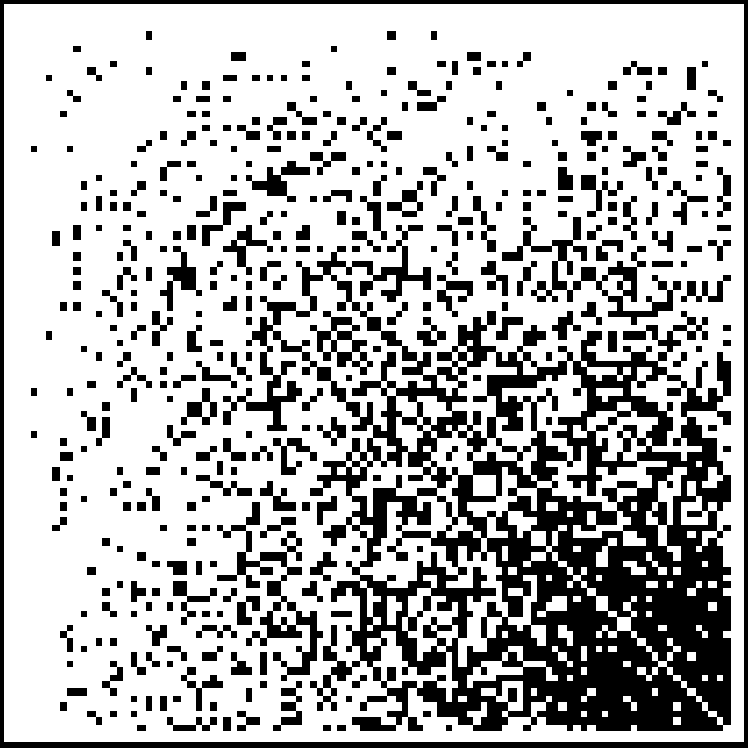
\includegraphics[width=0.18\columnwidth]{../misc/lovasz_sample100.pdf}
    %\includegraphics[width=2.8cm]{include/uniform_attachment_empirical.pdf}
  };
  \end{scope}
\end{tikzpicture}

%\end{center}

\mysection{Section 2c}

\vspace{0\baselineskip}

{\Large

%\begin{itemize}
%\item Inducing points in subset of regressors appoximation treated as random variables (locations and values)
%\item Gaussian process sampled using elliptical slice sampling; all other parameters sampled using slice sampling
%\end{itemize}

}

%\mysection{Inference: random inducing points}
%
%\newcommand{\numobs}{\mathrm O}
%\newcommand{\numnodes}{\mathrm N}
%
%For tractability, we apply a variation of a method known as Subsets-of-Regressors (SoR).
%The SoR approximation replaces the infinite dimensional GP with a finite dimensional approximation.
%Our approach is to treat both the inputs and outputs of the GP as latent variables.
%
%In particular, we introduce $k$ Gaussian distributed pseudoinputs $\pseudopoints=(\pseudopoints_1,\dotsc,\pseudopoints_k)$
%and define target values ${\targets_j = \AHfunction(\pseudopoints_j)}$.
%Writing $K_{\pseudopoints\pseudopoints}$ for the kernel matrix formed from the pseudoinputs $\pseudopoints$, we have
%\[
%(\pseudopoints_i) \simiid \Normal(0,I_{2r}) \qquad\text{and}\qquad
%\targets \given \pseudopoints \dist \Normal(0,K_{\pseudopoints\pseudopoints}).
%\]
%The idea of the SoR approximation is to replace $\larray_{ij}$ with the posterior mean conditioned on $(\pseudopoints,\targets)$,
%\[
%\larray = K_{\inputpoints\pseudopoints} K_{\pseudopoints\pseudopoints}^{-1}\targets,
%\label{eqn:GPConditional}
%\]
%where $K_{\inputpoints\pseudopoints}$ is the kernel matrix between the latent embeddings $\inputpoints$ and the pseudoinputs $\pseudopoints$.  By considering random pseudoinputs, we construct an MCMC analogue of other methods in the literature.
%
%Inference then performed using slice sampling and elliptical slice sampling.

\newpage

\mysection{Ising Model: Single-site Gibbs vs. Parallel Tempering}

\vspace{0.5\baselineskip}

%\begin{center}
%  \begin{tikzpicture}
  \begin{scope}[xshift=0cm]
    \node [mybox] (box){
      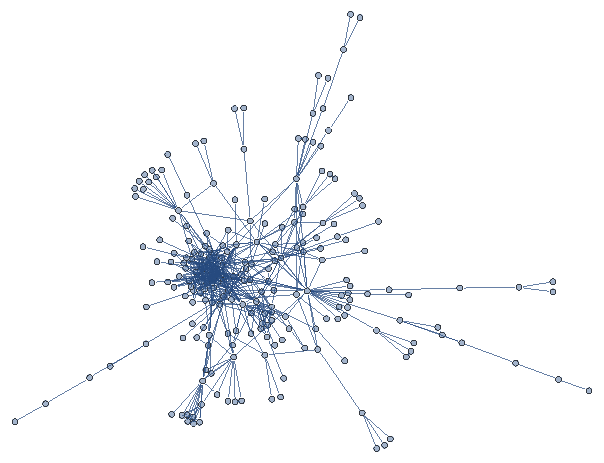
\includegraphics[width=0.1\textwidth]{../misc/graph_standard.pdf}
    };
    \node[inner sep=0,text width=0.1\textwidth, text centered] (note1) at (0,-0.06\textwidth) {
         A protein interactome};
  \end{scope}
  \begin{scope}[xshift=0.10\textwidth]
    \node [mybox] (box){
      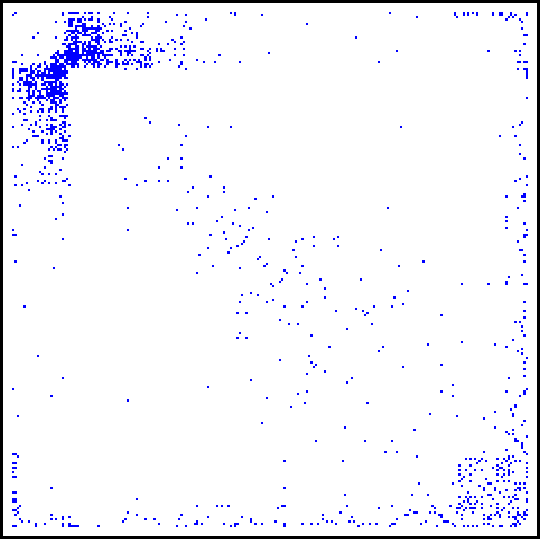
\includegraphics[width=0.08\textwidth]{../misc/interactome_adjacency_mathematica.pdf}
  };
    \node[inner sep=0,text width=0.1\textwidth, text centered] (note1) at (0,-0.06\textwidth) {
         Adjacency matrix sorted by MAP embedding};
  \end{scope}  
  \begin{scope}[xshift=0.20\textwidth]
    \node [mybox] (box){
      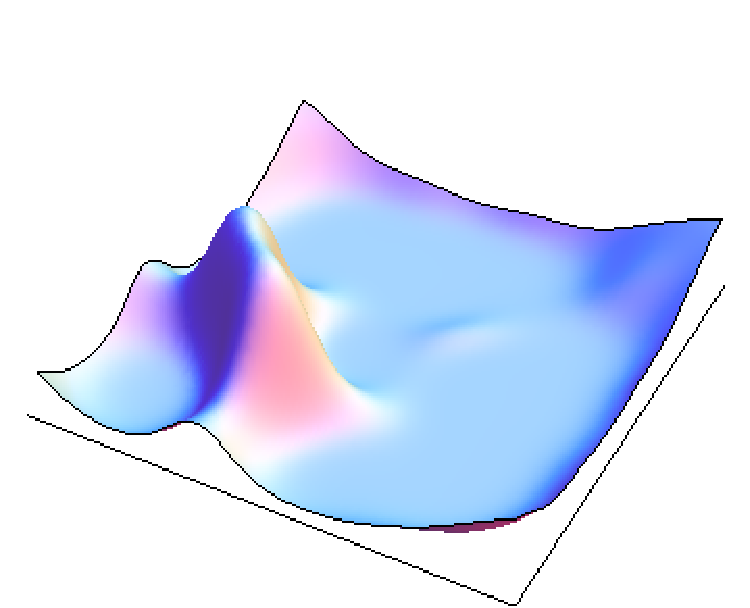
\includegraphics[width=0.1\textwidth]{../misc/graphon_listplot_bmp.pdf}
  };
    \node[inner sep=0,text width=0.1\textwidth, text centered] (note1) at (0,-0.06\textwidth) {
         MAP $\Theta$};
  \end{scope}
\end{tikzpicture}

%\end{center}

\vspace{\baselineskip}

%Sorting the adjacency matrix of the protein interactome using the (approximate) MAP values of the $\AHvar_i$ reveals interpretable structure in the data.
%The higher density of edges along the diagonal reveals homophily.
%The block structure in the top left reveals stochastic equivalence.
%These features can also be seen in the MAP $\Theta$.

\vspace{0.5\baselineskip}

\mysection{Hamiltonian Monte Carlo}

\vspace{\baselineskip}

%\begin{center}
%  \begin{tabular}{lccl} 
%%    \toprule
%    \multicolumn{4}{c}{Graph data}\\
%    \midrule
%    %\addlinespace[2pt]
%    %\textcolor{red}{Random function model} 
%    Random function model & $\AHfunction$ & $\sim$ & $\GP\,(0, \kernel)$\\
%    Latent class & $\larray_{ij}$ & $=$ & $\Lambda_{\AHvar_i\AHvar_j}\,\textrm{where} \,\AHvar_i \in \{1,\ldots,K\}$\\
%    IRM & $\larray_{ij}$ & $=$ & $\Lambda_{\AHvar_i\AHvar_j}\,\textrm{where} \,\AHvar_i \in \{1,\ldots,\infty\}$\\
%    Latent distance & $\larray_{ij}$ & $=$ & $-|\AHvar_i - \AHvar_j|$\\
%    Eigenmodel &$\larray_{ij}$ & $=$ & $\AHvar_i'\Lambda \AHvar_j$\\
%    LFRM & $\larray_{ij}$ & $=$ & $\AHvar_i'\Lambda \AHvar_j\,\textrm{where} \,\AHvar_i \in \{0,1\}^\infty$\\
%    ILA & $\larray_{ij}$ & $=$ & $\sum_d \mathbb{I}_{U_{id}}\mathbb{I}_{U_{jd}}\Lambda^{(d)}_{U_{id}U_{jd}}\,\textrm{where} \,\AHvar_i \in \{0,\ldots,\infty\}^\infty$\\
%    SMGB & $\AHfunction$ & $\dist$ & $\GP\,(0, \kernel_1 \otimes \kernel_2)$ \\
%    %\midrule
%    \addlinespace[4pt]
%    \multicolumn{4}{c}{Real-valued array data}\\
%    \midrule
%    %\textcolor{red}{Random function model} 
%    Random function model & $\AHfunction$ & $\sim$ & $\GP\,(0, \kernel)$\\
%    Mondrian process based & $\AHfunction$ & = & piece-wise constant random function\\
%    PMF & $\larray_{ij}$ & $=$ & $\AHvar_i'V_j$\\
%    GPLVM & $\AHfunction$ & $\sim$ & $\GP\,(0, \kernel \otimes \delta)$\\
%    %Linear relational GP~\cite{Yu2008} & $\AHfunction$ & $\sim$ & $\GP\,(0, \kernel_1 \otimes \kernel_2)\,\textrm{where} \,\kernel_i\,\textrm{is linear} $\\
%%\bottomrule
%\end{tabular}
%\end{center}

\vspace{\baselineskip}

\mysection{Code and References}

\vspace{\baselineskip}

%\begin{center}
%  \begin{tabular}{r | r r r | r r r | r r r}
%    \multicolumn{10}{c}{AUC results} \\
%    \addlinespace[2pt]
%    Data set & \multicolumn{3}{c|}{High school} & \multicolumn{3}{c|}{NIPS} & \multicolumn{3}{c}{Protein} \\
%    Latent dim. & 1 & 2 & 3 & 1 & 2 & 3 & 1 & 2 & 3 \\
%    \midrule
%    PMF                   & 0.747 & 0.792 & 0.792 & 0.729 & 0.789 & 0.820 & 0.787 & 0.810 & 0.841 \\
%    Eigenmodel            & 0.742 & 0.806 & 0.806 & 0.789 & 0.818 & 0.845 & 0.805 & 0.866 & 0.882 \\
%    GPLVM                 & 0.744 & 0.775 & 0.782 & 0.888 & 0.876 & 0.883 & 0.877 & 0.883 & 0.873 \\
%    RFM & \textbf{0.815} & \textbf{0.827} & \textbf{0.820} & \textbf{0.907} & \textbf{0.914} & \textbf{0.919} & \textbf{0.903} & \textbf{0.910} & \textbf{0.912}
%  \end{tabular}
%\end{center}

%\small{
%\bibliographystyle{unsrt}
%\bibliographystyle{../misc/natbib}
%\bibliography{misc/library,misc/biblio,misc/bibdesk-porbanz}
%}

\end{multicols}

\end{poster}

\end{document}
